% Introduction

% Main chapter title
\chapter{Introduction} 

% Change X to a consecutive number; for referencing this chapter elsewhere, use \ref{ChapterX}
%*******************************************************************************
%*********************************** First Chapter *****************************
%*******************************************************************************



\ifpdf
    \graphicspath{{Chapter1/Figs/Raster/}{Chapter1/Figs/PDF/}{Chapter1/Figs/}}
\else
    \graphicspath{{Chapter1/Figs/Vector/}{Chapter1/Figs/}}
\fi


%********************************** %First Section  **************************************
Speech processing and recognition have entered an exciting phase with voice-recognition application becoming ubiquitous across platforms. A prerequisite to capture any speech from the surroundings is the microphone. For many applications like video conferencing, and interactive home devices, the distance of the microphone from the speaker can be a few meters. Further processing or use of these speech signals, recorded from a distance is a challenge for two reasons. First, since the strength of the speech signal attenuates with distance, the background noise is more prominent in the recorded audio, than it would be for a close distance recording and proves obtrusive in recognition. Also, the speech signal may be reflected from multiple surfaces in the surroundings and cause an echo like effect in the recorded signal. This latter phenomenon is called Reverberation. Although, the human brain handles the effects of reverberation quite well, it severely distorts automatic speech recognizers’ capability to understand speech. \\

\section{Reverberation model}
Reverberation happens when an audio signal, after emanating from the source, undergoes multiple reflections from the surfaces in room. These reflections persist even when the source is switched off. The amount and nature of reverberation introduced in the speech signal depend on the surroundings in which the recording is done, as well as the relative positions of the microphone and the speaker. The degree of reverberation introduced by a particular enclosure or surrounding can be measured by the reverberation time (RT), also known as the T60. The Reverberation time is the time it takes for the signal strength to fall 60 db at the microphone, after the source is switched off. It is a characteristic property of the enclosure or environment where the source signal is recorded. Figure \ref{Reverberation} is an illustration of the mechanism of the process that leads to reverberation. In signal processing, the phenomenon of reverberation can be modeled as convolution of the source signal, $s(t)$ with a filter, $h(t)$.
\begin{align}
y(t) = s(t)*h(t) \label{eq :1}
\end{align}


Where $h(t)$ is the impulse response of the environment in which the source signal, $s(t)$ was generated and it depends on the relative positions of the microphone and the source and also the surroundings in which the signal is recorded. 

\begin{figure}[h]
\centering
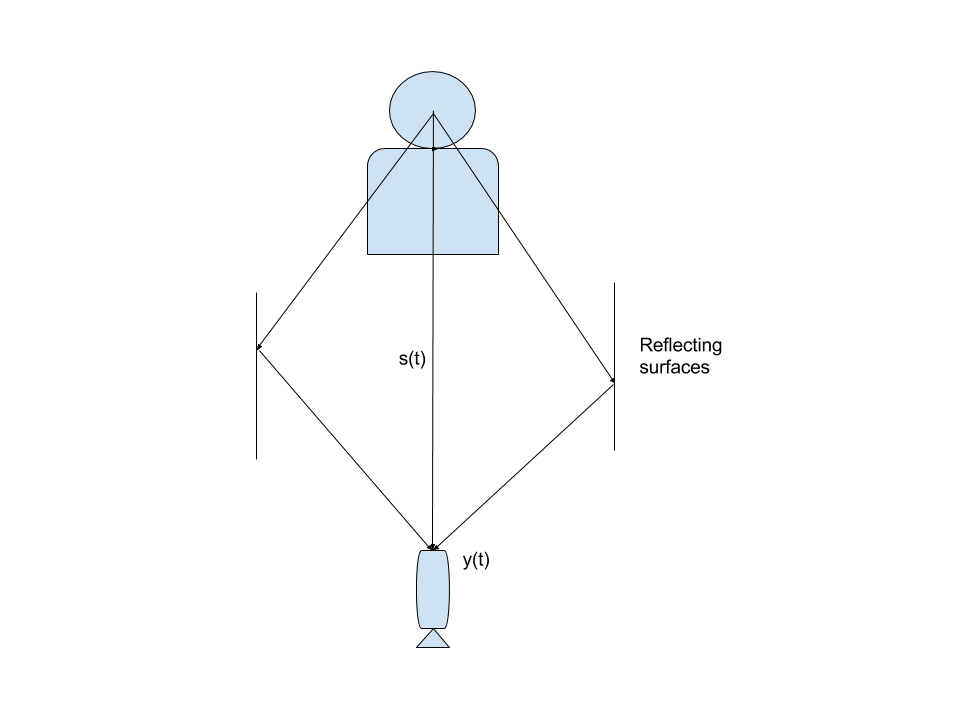
\includegraphics[scale=0.35]{Reverberation} 
\caption{The reason for reverberation. Along with the source signal, several of its reflections from nearby surfaces are also recorded by the microphone}\label{Reverberation}
\end{figure}

An example of a room impulse response is shown in Figure \ref{rir}. Each peak in the figure corresponds to a reflection arriving at the microphone after the original signal has arrived. Clearly there are a series of prominent reflections, temporally close to the direct signal(which arrived at time t=0), followed by weaker reflections which persist, at time up to 1000ms after the direct signal has died down. The reverberation time for typical office or home environments ranges from 200ms to 1000ms.  

\begin{figure}
\centering
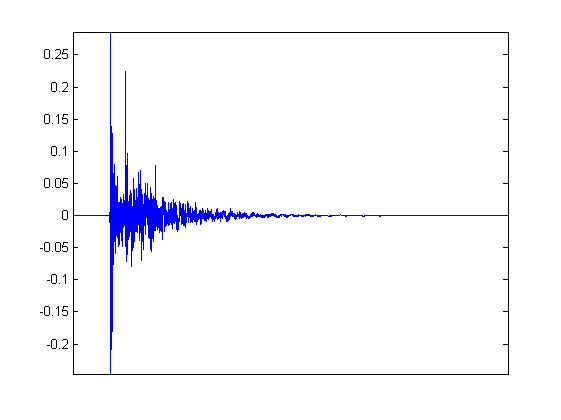
\includegraphics[scale=0.7]{rir} \label{rir}
\caption{An example of a typical time domain room impulse response. The strength of the reflections decays with time }\label{rir}
\end{figure}


\section{Automatic speech recognition and reverberation}
The aim of this section is to give an overview of  an automatic recognition system. It will also describe the broad categories of dereverberation techniques. 
Figure \ref{asr}  shows the schematic of a typical automatic speech recognizer. The goal of the recognition process is to transcribe speech correctly into text. This whole process can be divided into two stages - the front end and the back end.

\begin{figure}
\centering
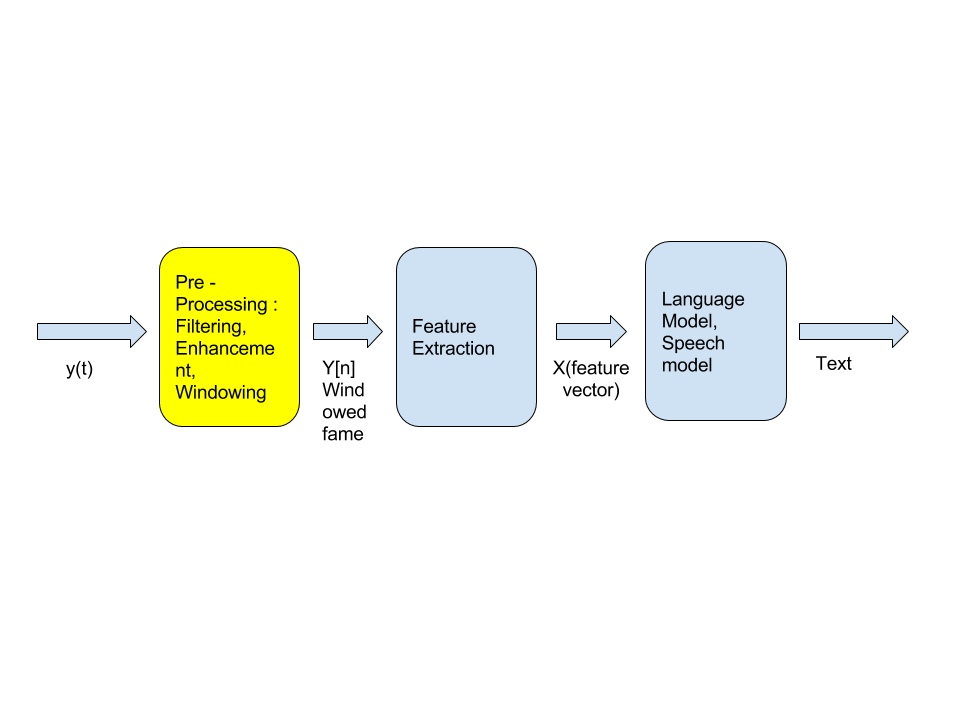
\includegraphics[scale=0.35]{asr} 
\caption{Schematic of an ASR system. All algorithms discussed here are applicable to the Pre-processing stage }\label{asr}
\end{figure}

At the front end, necessary pre-processing is done to extract useful information for further processing and making the speech signal more compact by discarding irrelevant information and noise. The pre-processing stage attempts to make the incoming speech as independent of the room acoustics and the speaker, as possible for easy recognition. The common steps carried out at this stage are sampling, windowing, denoising and speech enhancement. 

The next critical step is feature extraction from the windowed and enhanced speech. Some information in the speech signal is not relevant to the recognition process. Thus, relevant features have to be extracted from the windowed signal. Furthermore, selecting a few features also reduces the dimensionality of the input data reducing computation time. Some prominent features such as the Mel-Cepstral features and wavelet domain features are used in almost all modern ASR applications. These features are extracted from windowed time frames of upto 40ms because of the quasi-stationary nature of speech in that time frame. That is, each segment of speech that is , say for instance, 30ms long is used to extract one feature vector.

After the incoming speech has been converted into a feature vector $X$, the ASR system has to estimate the sequence of words $w$, that would have given rise to $X$. It is here that acoustic and language models for speech are deployed. An acoustic model can, given a feature vector, predict the sound or phoneme that was uttered by the speaker and the language model provides the understanding of the language i.e. a probability distribution over sequences of words.
Mathematically, after the the signal $y(t)$ has been converted into a feature vector $x_{n \in T}$, where $T$ is the temporal the ASR system arrives at the correct transcription by solving the equation
\begin{align}
w^{*} = argmax_w p((X_n)_{n\in T} )p(w)
\end{align}
Here, p(w) gives the likelihood of observing $w$ in the present sequence of words and comes from the language model. $p((X_n)_{n\in T} )$, on the other hand quantifies the likelihood that $X$ would be observed, if $w$ was indeed spoken. This comes from the acoustic model.
\\

As mentioned earlier, the performance of the system depends on the quality of the features extracted. Typically, features are extracted from windowed segment of speech of length of 10-40ms because of quasi-stationary nature of speech in that duration. On the other hand, reverberation, as we have seen, can have deteriorating effects on the quality of speech, and thus the features extracted for upto 1000ms. This means that the impact of reverberation can last several frames. This poses a unique challenge and cannot be addressed like ordinary noise which is not correlated beyond a few ms.
\begin{figure}[H]
\centering
\begin{minipage}{.5\textwidth}
  \centering
  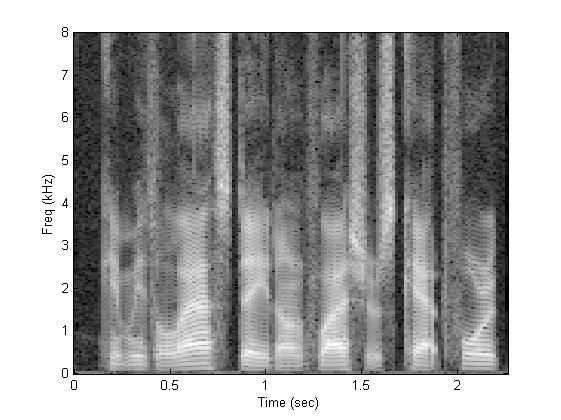
\includegraphics[width=.9\linewidth]{clean} 
  \captionof{figure}{Magnitude spectrogram of a speech signal without any reverberation}\label{clean_ch1}
\end{minipage}%
\begin{minipage}{.5\textwidth}
  \centering
  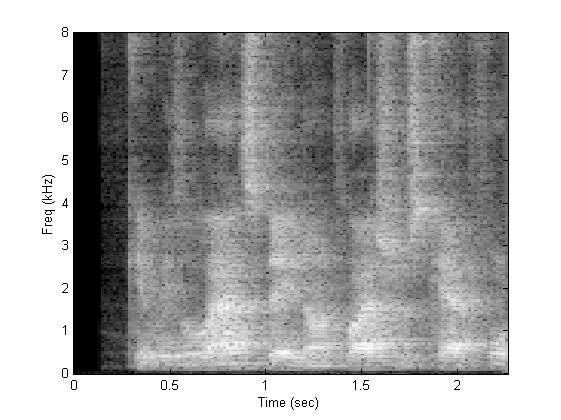
\includegraphics[width=.9\linewidth]{input_normal} 
  \captionof{figure}{Magnitude spectrogram of the speech signal with reverberation.  }\label{input_normal_ch1}
\end{minipage}
\end{figure}

Figure\ref{clean_ch1} and \ref{input_normal_ch1} show the effect of reverberation on the magnitude spectrogram of a speech signal due to reverberation. Clearly, there is a ‘smearing’ effect, apparent in the magnitude domain as well as the feature domain. The reverberation caused by a single segment of speech can distort features for several subsequent frames, depending on the Reverberation Time. This distortion of features causes the ASR to function sub-optimally. Techniques to tackle noise cannot be directly deployed to tackle this since reverberation distortion is non-stationary as well as correlated with the real speech signal.

The ways to tackle reverberation can be separated into two broad approaches - front end and back end approaches. Front end approaches aim at cleaning the reverberation away from the feature vectors which can then be fed into the back-end of the speech recognition system, which works as it does for clean speech. Back-end techniques on the other hand aim at changing the acoustic model or change the decoding scheme for the feature vectors to account for reverberation. 

Here, the focus is only going to be on front end based approaches. Further, although the choice of features to be extracted is a critical component of the recognition process, that line of investigation is not explored here. Since majority of the features are derived from the magnitude-spectrum of the speech signal (eg. MFCC coefficients), only those techniques which propose to enhance and remove the effects of reverberation the magnitude spectrum have been explored. The phase information will be discarded in all the following investigations from the spectrogram. This has an added advantage of making the processing independent of speaker movement  since slight movements will only change the phase of the spectrogram.

Also, it will be hereon assumed that only a single microphone is used for the recording, and no prior information about the speaker, the surroundings or the microphone is known. Thus the exact problem that is going to be addressed is Single Channel Blind Dereverberation. 

However, much work has been done on modeling speech. There are a few universal properties that apply to all speech signals. We will put these properties to use to model clean speech better and thus improve dereverberation performance for some algorithms. Although, the room impulse response in much more difficult to model, a few simplifying assumptions will be made.

The next chapter, Chapter 2 will conceptually describe Non-Negative matrix factorization(NMF) and its application to speech processing. Chapter 3 discusses popular dereverberation techniques and how NMF factorization of speech magnitude spectrograms can improve the efficiency of these algorithms. 








